\documentclass[11pt,a4paper]{report}
\usepackage[textwidth=37em,vmargin=30mm]{geometry}
\usepackage{calc,xunicode,amsmath,amssymb,paralist,enumitem,tabu,booktabs,datetime2,xeCJK,xeCJKfntef,listings}
\usepackage{tocloft,fancyhdr,tcolorbox,xcolor,graphicx,eso-pic,xltxtra,xelatexemoji}

\newcommand{\envyear}[0]{2025}
\newcommand{\envdatestr}[0]{2025-08-17}
\newcommand{\envfinaldir}[0]{webdb/2025/20250817/final}

\usepackage[hidelinks]{hyperref}
\hypersetup{
    colorlinks=false,
    pdfpagemode=FullScreen,
    pdftitle={Web Digest - \envdatestr}
}

\setlength{\cftbeforechapskip}{10pt}
\renewcommand{\cftchapfont}{\rmfamily\bfseries\large\raggedright}
\setlength{\cftbeforesecskip}{2pt}
\renewcommand{\cftsecfont}{\sffamily\small\raggedright}

\setdefaultleftmargin{2em}{2em}{1em}{1em}{1em}{1em}

\usepackage{xeCJK,xeCJKfntef}
\xeCJKsetup{PunctStyle=plain,RubberPunctSkip=false,CJKglue=\strut\hskip 0pt plus 0.1em minus 0.05em,CJKecglue=\strut\hskip 0.22em plus 0.2em}
\XeTeXlinebreaklocale "zh"
\XeTeXlinebreakskip = 0pt


\setmainfont{Brygada 1918}
\setromanfont{Brygada 1918}
\setsansfont{IBM Plex Sans}
\setmonofont{JetBrains Mono NL}
\setCJKmainfont{Noto Serif CJK SC}
\setCJKromanfont{Noto Serif CJK SC}
\setCJKsansfont{Noto Sans CJK SC}
\setCJKmonofont{Noto Sans CJK SC}

\setlength{\parindent}{0pt}
\setlength{\parskip}{8pt}
\linespread{1.15}

\lstset{
	basicstyle=\ttfamily\footnotesize,
	numbersep=5pt,
	backgroundcolor=\color{black!5},
	showspaces=false,
	showstringspaces=false,
	showtabs=false,
	tabsize=2,
	captionpos=b,
	breaklines=true,
	breakatwhitespace=true,
	breakautoindent=true,
	linewidth=\textwidth
}






\newcommand{\coverpic}[2]{
    % argv: itemurl, authorname
    Cover photo by #2~~(\href{#1}{#1})
}
\newcommand{\makeheader}[0]{
    \begin{titlepage}
        % \newgeometry{hmargin=15mm,tmargin=21mm,bmargin=12mm}
        \begin{center}
            
            \rmfamily\scshape
            \fontspec{BaskervilleF}
            \fontspec{Old Standard}
            \fontsize{59pt}{70pt}\selectfont
            WEB\hfill DIGEST
            
            \vfill
            % \vskip 30pt
            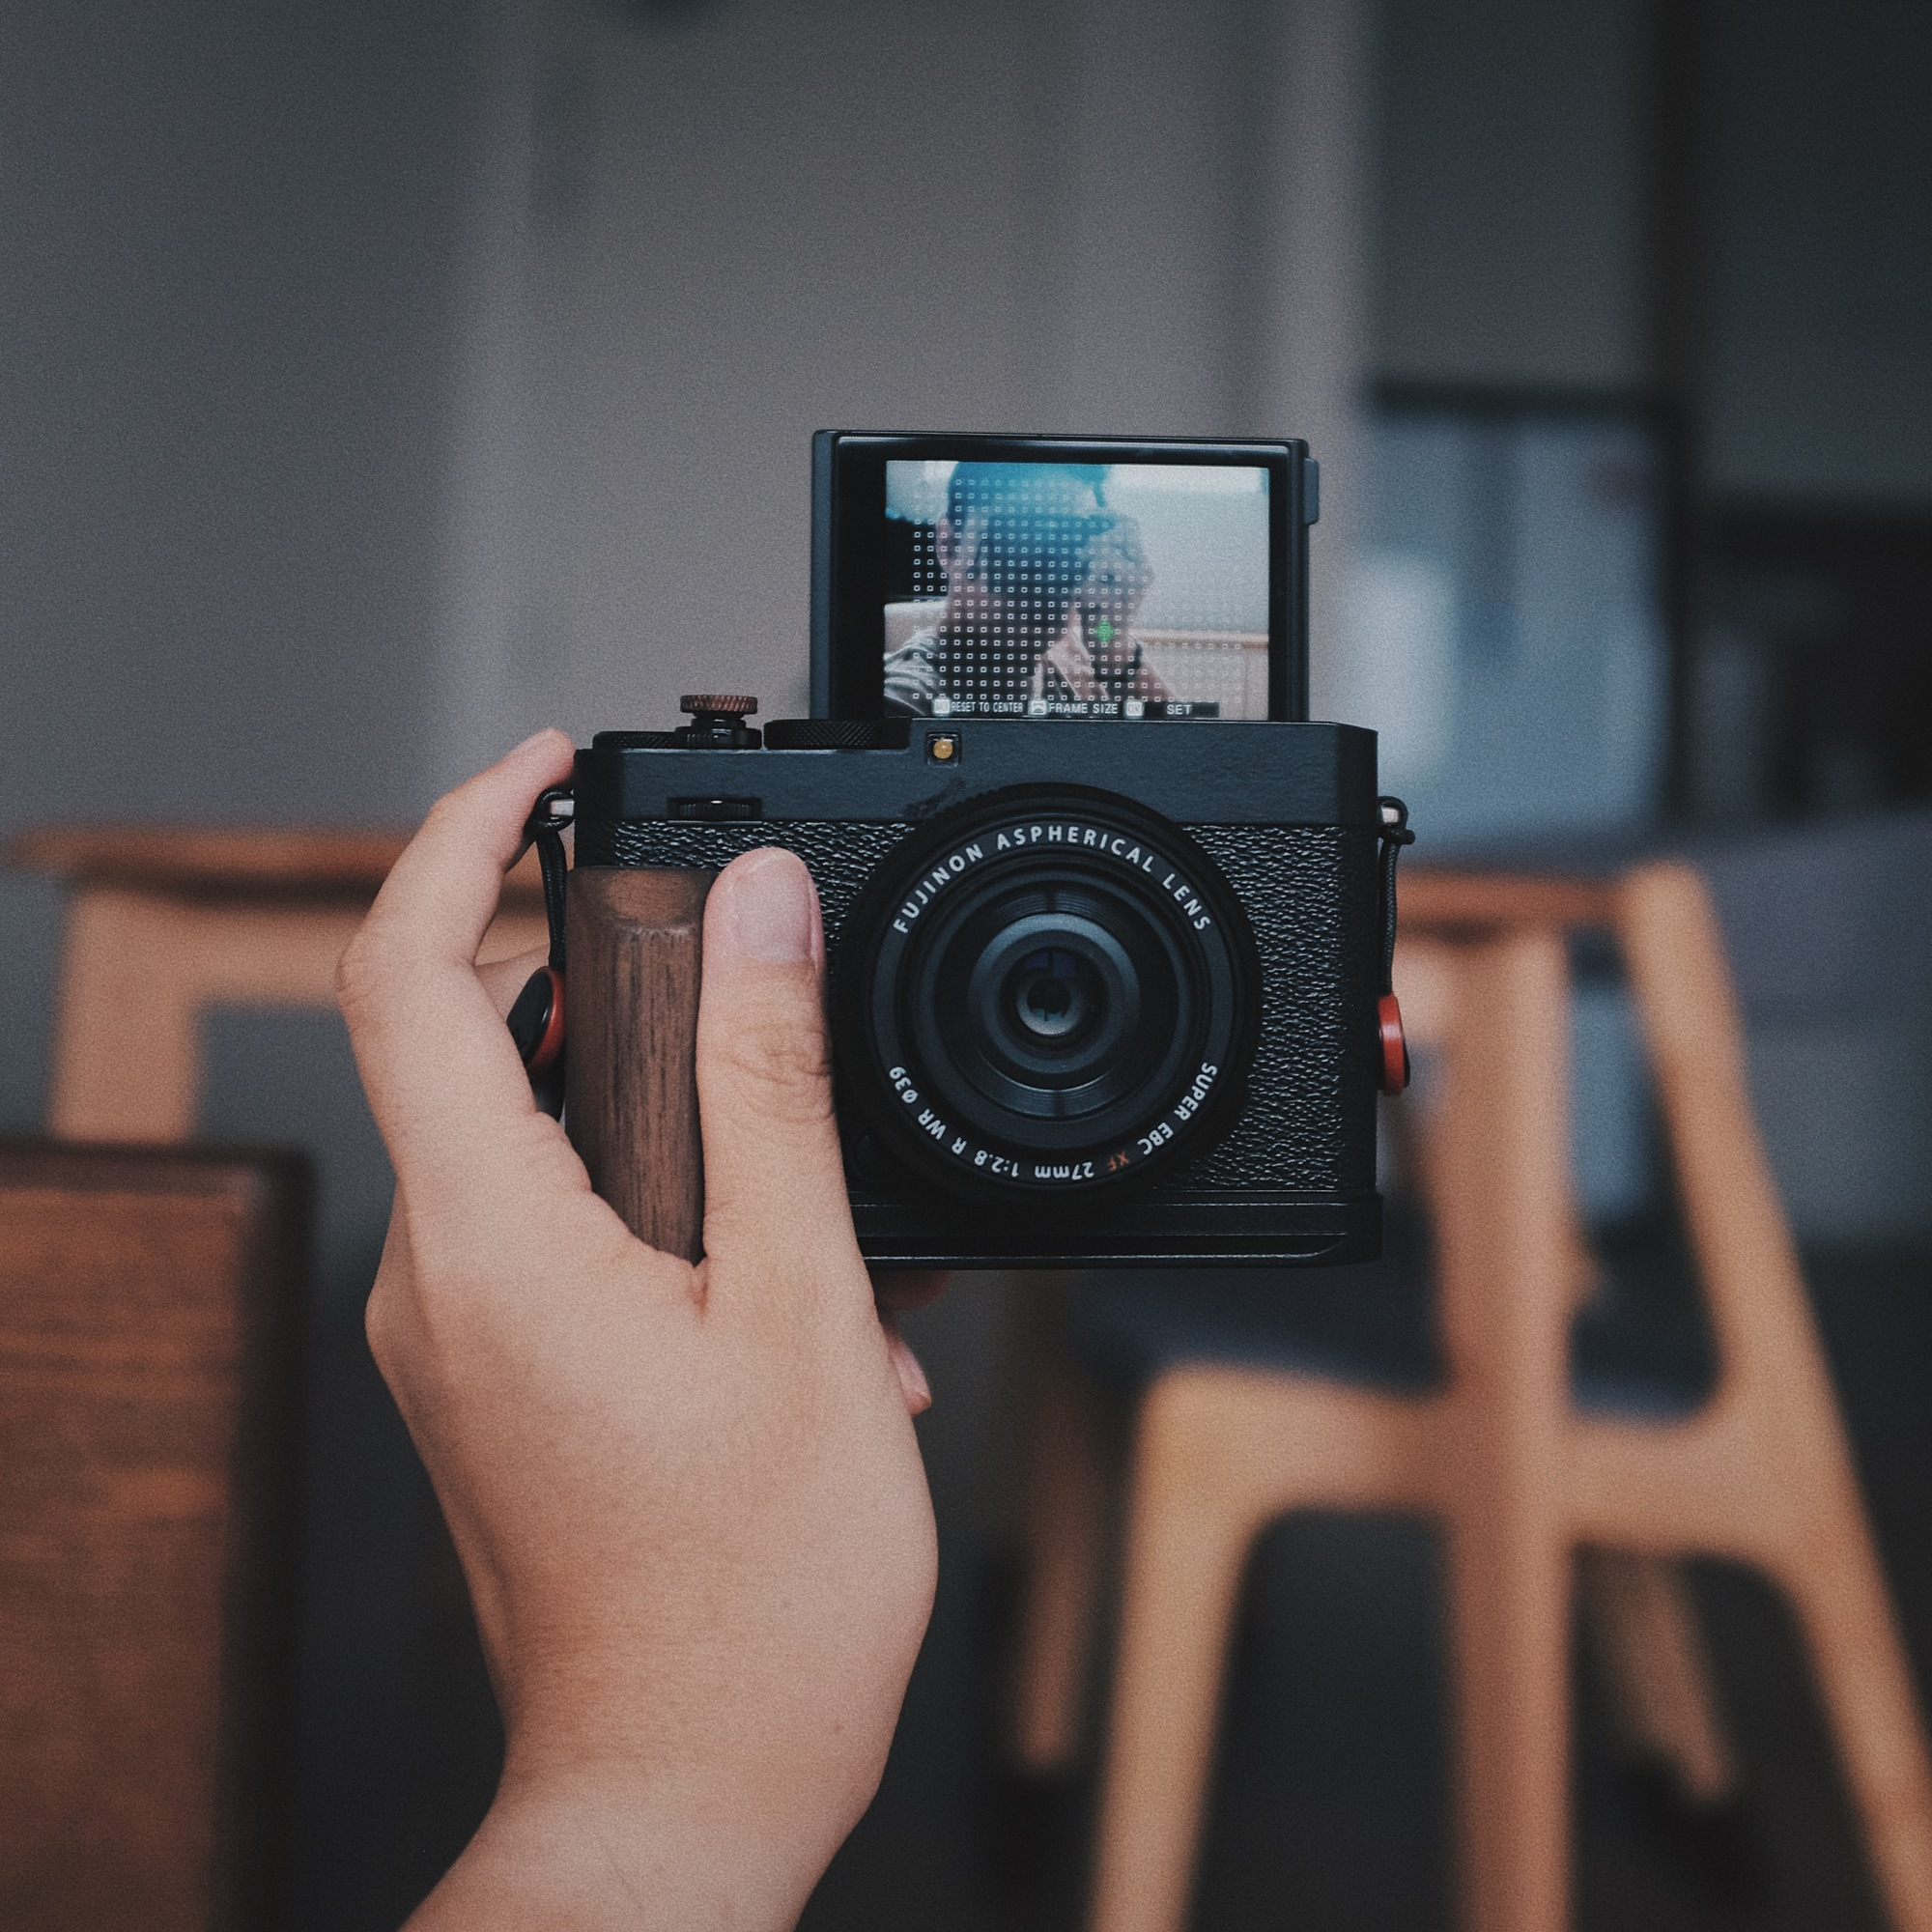
\includegraphics[width=\linewidth]{\envfinaldir/coverpic-prod.jpg}\par
            % \vskip 30pt
            \vfill

            \normalsize\rmfamily\scshape
            \copyright{} The Web Digest Project \hfill\large \envdatestr
        \end{center}
    \end{titlepage}
    % \restoregeometry
}
\newcommand{\simplehref}[1]{%
    \textcolor{blue!80!green}{\href{#1}{#1}}%
}
\renewcommand{\contentsname}{\center\Huge\sffamily\bfseries Contents\par\vskip 20pt}
\newcounter{ipartcounter}
\setcounter{ipartcounter}{0}
\newcommand{\ipart}[1]{
    % \vskip 20pt
    \clearpage
    \stepcounter{ipartcounter}
    \phantomsection
    \addcontentsline{toc}{chapter}{#1}
    % \begin{center}
    %     \Huge
    %     \sffamily\bfseries
    %     #1
    % \end{center}
    % \vskip 20pt plus 7pt
}
\newcounter{ichaptercounter}
\setcounter{ichaptercounter}{0}
\newcommand{\ichapter}[1]{
    % \vskip 20pt
    \clearpage
    \stepcounter{ichaptercounter}
    \phantomsection
    \addcontentsline{toc}{section}{\numberline{\arabic{ichaptercounter}}#1}
    \begin{center}
        \Huge
        \sffamily\bfseries
        #1
    \end{center}
    \vskip 20pt plus 7pt
}
\newcommand{\entrytitlefont}[1]{\subsection*{\raggedright\Large\sffamily\bfseries#1}}
\newcommand{\entryitemGeneric}[2]{
    % argv: title, url
    \parbox{\linewidth}{
        \entrytitlefont{#1}\par\vskip 5pt
        \footnotesize\ttfamily\mdseries
        \simplehref{#2}
    }\vskip 11pt plus 11pt minus 1pt
}
\newcommand{\entryitemGithub}[3]{
    % argv: title, url, desc
    \parbox{\linewidth}{
        \entrytitlefont{#1}\par\vskip 5pt
        \footnotesize\ttfamily\mdseries
        \simplehref{#2}\par\vskip 5pt
        \small\rmfamily\mdseries#3
    }\vskip 11pt plus 11pt minus 1pt
}
\newcommand{\entryitemAp}[3]{
    % argv: title, url, desc
    \parbox{\linewidth}{
        \entrytitlefont{#1}\par\vskip 5pt
        \footnotesize\ttfamily\mdseries
        \simplehref{#2}\par\vskip 5pt
        \small\rmfamily\mdseries#3
    }\vskip 11pt plus 11pt minus 1pt
}
\newcommand{\entryitemHackernews}[3]{
    % argv: title, hnurl, rawurl
    % \parbox{\linewidth}{
    %     \entrytitlefont{#1}\par\vskip 5pt
    %     \footnotesize\ttfamily\mdseries
    %     \simplehref{#3}\par
    %     \textcolor{black!50}{\href{#2}{#2}}
    % }\vskip 11pt plus 11pt minus 1pt
    \begin{minipage}{\linewidth}
            \entrytitlefont{#1}\par\vskip 5pt
            \footnotesize\ttfamily\mdseries
            \simplehref{#3}\par
            \textcolor{black!50}{\href{#2}{#2}}
    \end{minipage}\par\vskip 11pt plus 11pt minus 1pt
}







\begin{document}

\makeheader

\tableofcontents\clearpage




\ipart{Developers}
\ichapter{Hacker News}
\entryitemTwoLinks{Claude Opus 4 and 4.1 can now end a rare subset of conversations}{https://news.ycombinator.com/item?id=44916813}{https://www.anthropic.com/research/end-subset-conversations}

\entryitemTwoLinks{Imagen 4 is now generally available}{https://news.ycombinator.com/item?id=44915187}{https://developers.googleblog.com/en/announcing-imagen-4-fast-and-imagen-4-family-generally-available-in-the-gemini-api/}

\entryitemTwoLinks{Show HN: Edka – Kubernetes clusters on your own Hetzner account}{https://news.ycombinator.com/item?id=44915164}{https://edka.io}

\entryitemTwoLinks{It seems like the AI crawlers learned how to solve the Anubis challenges}{https://news.ycombinator.com/item?id=44914773}{https://social.anoxinon.de/@Codeberg/115033790447125787}

\entryitemTwoLinks{Steam can't escape the fallout from its censorship controversy}{https://news.ycombinator.com/item?id=44914163}{https://www.polygon.com/steam-paypal-issues-censorship-visa-mastercard/}

\entryitemTwoLinks{Occult books digitized and put online by Amsterdam's Ritman Library}{https://news.ycombinator.com/item?id=44914061}{https://www.openculture.com/2025/08/2178-occult-books-now-digitized-put-online.html}

\entryitemTwoLinks{The electric fence stopped working years ago}{https://news.ycombinator.com/item?id=44913663}{https://soonly.com/electric-fences/}

\entryitemTwoLinks{Do Things That Don't Scale (2013)}{https://news.ycombinator.com/item?id=44913359}{https://paulgraham.com/ds.html}

\entryitemTwoLinks{The beauty of a text only webpage}{https://news.ycombinator.com/item?id=44913340}{https://albanbrooke.com/the-beauty-of-a-text-only-webpage/}

\entryitemTwoLinks{ADHD drug treatment and risk of negative events and outcomes}{https://news.ycombinator.com/item?id=44912861}{https://www.bmj.com/content/390/bmj-2024-083658}

\entryitemTwoLinks{The Timmy Trap}{https://news.ycombinator.com/item?id=44912646}{https://jenson.org/timmy/}

\entryitemTwoLinks{White House loyalty rating for companies}{https://news.ycombinator.com/item?id=44912369}{https://www.axios.com/2025/08/15/white-house-rating-big-beautiful-bill}

\entryitemTwoLinks{Is Germany on the brink of banning ad blockers?}{https://news.ycombinator.com/item?id=44912085}{https://blog.mozilla.org/netpolicy/2025/08/14/is-germany-on-the-brink-of-banning-ad-blockers-user-freedom-privacy-and-security-is-at-risk/}

\entryitemTwoLinks{Vaultwarden commit introduces SSO using OpenID Connect}{https://news.ycombinator.com/item?id=44911560}{https://github.com/dani-garcia/vaultwarden/pull/3899}

\entryitemTwoLinks{Open hardware desktop 3D printing is dead?}{https://news.ycombinator.com/item?id=44911423}{https://www.josefprusa.com/articles/open-hardware-in-3d-printing-is-dead/}

\entryitemTwoLinks{Fairness is what the powerful 'can get away with' study shows}{https://news.ycombinator.com/item?id=44911169}{https://phys.org/news/2025-07-fairness-powerful.html}

\entryitemTwoLinks{Court records reveal Sig Sauer knew of pistol risks for years}{https://news.ycombinator.com/item?id=44911069}{https://smokinggun.org/court-records-reveal-sig-sauer-knew-of-pistol-risks-for-years/}

\entryitemTwoLinks{Swiss vs. UK approach to major tranport projects}{https://news.ycombinator.com/item?id=44910393}{https://www.freewheeling.info/blog/swiss-hs2}

\entryitemTwoLinks{UK government states that 'safety' act is about influence over public discourse}{https://news.ycombinator.com/item?id=44910161}{https://bsky.app/profile/tupped.bsky.social/post/3lwgcmswmy222}

\entryitemTwoLinks{Simulating and Visualising the Central Limit Theorem}{https://news.ycombinator.com/item?id=44909133}{https://blog.foletta.net/post/2025-07-14-clt/}\ichapter{Phoronix}
\entryitemGeneric{\hskip 0pt{}Linux 6.16.1 Fixes A Large Intel GPU Driver Performance Regression - Up To 30\%}{https://www.phoronix.com/news/Linux-6.16.1-Fixes-Intel-i915}

\entryitemGeneric{\hskip 0pt{}GNOME Disks Continues Being Ported To Rust}{https://www.phoronix.com/news/GNOME-Disks-More-Rust}

\entryitemGeneric{\hskip 0pt{}Wine-Staging 10.13 Adds Patch For 13 Year Old Bug}{https://www.phoronix.com/news/Wine-Staging-10.13}

\entryitemGeneric{\hskip 0pt{}KDE Breeze Drops Colorful Third-Party App Icons, Plasma Adds Plug-In Device Notification}{https://www.phoronix.com/news/KDE-Plug-In-Device-Notification}

\entryitemGeneric{\hskip 0pt{}GNOME 49 Beta Ships Many Last Minute Features - Including Greater systemd Reliance}{https://www.phoronix.com/news/GNOME-49-Beta}

\entryitemGeneric{\hskip 0pt{}Linux 6.17 Features: Great Intel Graphics Improvements, AMD HFI, Attack Vector Controls + Lenovo Gaming Drivers}{https://www.phoronix.com/review/linux-617-features}

\entryitemGeneric{\hskip 0pt{}Wine 10.13 Released With One Month Worth Of Improvements}{https://www.phoronix.com/news/Wine-10.13-Released}

\entryitemGeneric{\hskip 0pt{}Patches Posted For Raspberry Pi 5 Ethernet With The Upstream Linux Kernel}{https://www.phoronix.com/news/Raspberry-Pi-5-Ethernet-Linux}

\entryitemGeneric{\hskip 0pt{}Ubuntu Developing New "Dangerous" Desktop Images Concept}{https://www.phoronix.com/news/Ubuntu-Dangerous-Desktop}


\ipart{Developers~~~~(zh-Hans)}
\ichapter{Solidot}
\entryitemGeneric{\hskip 0pt{}PuTTY 有了新官网}{https://www.solidot.org/story?sid=82065}

\entryitemGeneric{\hskip 0pt{}德国最高法院部分推翻广告屏蔽工具不侵犯版权判决}{https://www.solidot.org/story?sid=82064}

\entryitemGeneric{\hskip 0pt{}维基百科历史上最大规模的自我推销行动}{https://www.solidot.org/story?sid=82063}

\entryitemGeneric{\hskip 0pt{}Google 发布紧凑型开源模型 Gemma 3 270M}{https://www.solidot.org/story?sid=82062}

\entryitemGeneric{\hskip 0pt{}退休后继续工作与更高的幸福度相关}{https://www.solidot.org/story?sid=82061}

\entryitemGeneric{\hskip 0pt{}半人马座 α 星可能存在一颗气态巨行星}{https://www.solidot.org/story?sid=82060}

\entryitemGeneric{\hskip 0pt{}特朗普政府考虑入股英特尔}{https://www.solidot.org/story?sid=82059}

\entryitemGeneric{\hskip 0pt{}现阶段的印度越南制造还只是中国加一}{https://www.solidot.org/story?sid=82058}

\entryitemGeneric{\hskip 0pt{}微软高管称语音将成为下一代 Windows 的主要输入方式}{https://www.solidot.org/story?sid=82057}

\entryitemGeneric{\hskip 0pt{}一氧化碳新解毒剂能在数分钟内清理血液}{https://www.solidot.org/story?sid=82056}

\entryitemGeneric{\hskip 0pt{}AI 数据中心推动美国居民电费全面上涨}{https://www.solidot.org/story?sid=82055}

\entryitemGeneric{\hskip 0pt{}广岛和长崎核爆幸存者死于辐射致癌的比例比预期的低}{https://www.solidot.org/story?sid=82054}

\entryitemGeneric{\hskip 0pt{}ReiserFS 在内核的最后残余被清除}{https://www.solidot.org/story?sid=82053}

\entryitemGeneric{\hskip 0pt{}俄罗斯限制 Telegram 和 WhatsApp 的语音呼叫功能}{https://www.solidot.org/story?sid=82052}

\entryitemGeneric{\hskip 0pt{}白宫考虑将对华销售收入上缴模式扩大到其它公司}{https://www.solidot.org/story?sid=82051}

\entryitemGeneric{\hskip 0pt{}DeepSeek 的 R2 模型因华为芯片问题推迟发布}{https://www.solidot.org/story?sid=82050}

\entryitemGeneric{\hskip 0pt{}美国年轻一代更喜欢加速播放视频和音频}{https://www.solidot.org/story?sid=82049}

\entryitemGeneric{\hskip 0pt{}中国推动开源模型令硅谷和华盛顿担忧}{https://www.solidot.org/story?sid=82048}

\entryitemGeneric{\hskip 0pt{}研究认为社交媒体的问题无法得到修正}{https://www.solidot.org/story?sid=82047}

\entryitemGeneric{\hskip 0pt{}挪威指责俄黑客破坏其水坝}{https://www.solidot.org/story?sid=82046}\ichapter{V2EX}
\entryitemGeneric{\hskip 0pt{}[程序员] go 写的 fzf 如何做到用比 rust 重写版快几倍}{https://www.v2ex.com/t/1152926}

\entryitemGeneric{\hskip 0pt{}[分享创造] showcase - 展示自己的 GitHub 项目,使用 GitHub Actions 自动更新并部署到 Pages}{https://www.v2ex.com/t/1152925}

\entryitemGeneric{\hskip 0pt{}[分享发现] 正在使用 lobe-chat 的朋友注意了! lobe-chat 正在泄漏你的隐私!}{https://www.v2ex.com/t/1152924}

\entryitemGeneric{\hskip 0pt{}[OpenAI] GPT5 非推理模型相对 GPT4.1 有什么优势}{https://www.v2ex.com/t/1152923}

\entryitemGeneric{\hskip 0pt{}[京东] 问下大家京东 PC 端网页版可以正常访问么?}{https://www.v2ex.com/t/1152922}

\entryitemGeneric{\hskip 0pt{}[Notion] notion offline 模式已经出来了?}{https://www.v2ex.com/t/1152921}

\entryitemGeneric{\hskip 0pt{}[互联网] 已经有域名想免费建个博客}{https://www.v2ex.com/t/1152920}

\entryitemGeneric{\hskip 0pt{}[问与答] 选官翻 iPad pro m1 12.9 还是全新 iPad pro m4 11}{https://www.v2ex.com/t/1152919}

\entryitemGeneric{\hskip 0pt{}[酷工作] 招聘在线课堂全栈开发(react + 云部署)}{https://www.v2ex.com/t/1152917}

\entryitemGeneric{\hskip 0pt{}[音乐] 求一个 80, 90 后网吧神曲歌单}{https://www.v2ex.com/t/1152916}

\entryitemGeneric{\hskip 0pt{}[程序员] 程序员应该怎么跟别人吵架?}{https://www.v2ex.com/t/1152915}

\entryitemGeneric{\hskip 0pt{}[OpenWrt] 求助: OpenWRT + AdGuard Home + OpenClash 配置 DNS 抗污染和去广告}{https://www.v2ex.com/t/1152914}

\entryitemGeneric{\hskip 0pt{}[Linux] 如何制作 Linux live cd}{https://www.v2ex.com/t/1152913}

\entryitemGeneric{\hskip 0pt{}[分享创造] [开源自荐] 轻量级的 HTML 组件模板引擎}{https://www.v2ex.com/t/1152911}

\entryitemGeneric{\hskip 0pt{}[硬件] 有木有人用过重力星球的鼠标,它这个脚贴是什么情况,怎么这么差🤣}{https://www.v2ex.com/t/1152910}

\entryitemGeneric{\hskip 0pt{}[奇思妙想] ``德州问题''}{https://www.v2ex.com/t/1152909}

\entryitemGeneric{\hskip 0pt{}[分享创造] [更新]SVGTOPNG 转换工具上线 1 月后的重大更新}{https://www.v2ex.com/t/1152908}

\entryitemGeneric{\hskip 0pt{}[问与答] 为什么 vaultwarden 要在 data 中存储私钥?}{https://www.v2ex.com/t/1152906}

\entryitemGeneric{\hskip 0pt{}[OpenWrt] 求教大佬们 N1 的 openwrt 的 clash 有时刷不出部分小红书 app 的图片}{https://www.v2ex.com/t/1152905}

\entryitemGeneric{\hskip 0pt{}[VPS] 各位安卓账号多的,你们都用什么 vps?}{https://www.v2ex.com/t/1152904}

\entryitemGeneric{\hskip 0pt{}[程序员] 有没有懂航旅纵横的}{https://www.v2ex.com/t/1152903}

\entryitemGeneric{\hskip 0pt{}[程序员] 咪咕体育的蛋疼 HDR...有没有在这上班的..}{https://www.v2ex.com/t/1152902}

\entryitemGeneric{\hskip 0pt{}[Solana] solana 功能求解}{https://www.v2ex.com/t/1152901}

\entryitemGeneric{\hskip 0pt{}[问与答] 二本应届生个人开发者产品求助:识图翻译类 App 优化与疑问}{https://www.v2ex.com/t/1152899}

\entryitemGeneric{\hskip 0pt{}[汽车] 被追尾后,对方认为修车费用太高,不肯支付怎么办?}{https://www.v2ex.com/t/1152898}

\entryitemGeneric{\hskip 0pt{}[分享发现] colemak vs norman 布局体验分享}{https://www.v2ex.com/t/1152896}

\entryitemGeneric{\hskip 0pt{}[酷工作] 上海招兼职 Flutter 工程师}{https://www.v2ex.com/t/1152895}

\entryitemGeneric{\hskip 0pt{}[微信] 关于微信 PC 4 版本的备份}{https://www.v2ex.com/t/1152894}

\entryitemGeneric{\hskip 0pt{}[问与答] 寻找一个以前听过的音乐}{https://www.v2ex.com/t/1152893}

\entryitemGeneric{\hskip 0pt{}[职场话题] 老哥们,现在广州 3 年后端开发什么行情啊}{https://www.v2ex.com/t/1152891}

\entryitemGeneric{\hskip 0pt{}[问与答] 请问 KE 改键中,如何禁用某个键?翻遍了官方手册没找到。我是外接的全尺寸键盘。}{https://www.v2ex.com/t/1152890}

\entryitemGeneric{\hskip 0pt{}[分享创造] DualPiP v1.1.0: 支持 Chrome 内置 AI 翻译,增强双语画中画体验}{https://www.v2ex.com/t/1152889}

\entryitemGeneric{\hskip 0pt{}[随想] 你们可以找一个比较大的数,让大模型判断一下是不是质数}{https://www.v2ex.com/t/1152888}

\entryitemGeneric{\hskip 0pt{}[Solana] Ledger 的 Solana 目前无法 signMessage,绑定逻辑是否可以增加一种:交易 + Memo 来替代}{https://www.v2ex.com/t/1152886}

\entryitemGeneric{\hskip 0pt{}[Solana] 教程:如何让空投能砸中你呢?}{https://www.v2ex.com/t/1152885}

\entryitemGeneric{\hskip 0pt{}[前端开发] 现在如果手搓一个学校政务官网,支持低版本 IE 的话,现在推荐什么技术栈?}{https://www.v2ex.com/t/1152884}

\entryitemGeneric{\hskip 0pt{}[Claude] 有 cluade-pro,在国内如何使用 claude code}{https://www.v2ex.com/t/1152878}

\entryitemGeneric{\hskip 0pt{}[问与答] 一种门窗报警器, 24 小时未打开门即亮灯提醒。}{https://www.v2ex.com/t/1152877}

\entryitemGeneric{\hskip 0pt{}[问与答] github repo 上的 Open with xxx 以前好像看到过 Idea,但是现在没了}{https://www.v2ex.com/t/1152876}

\entryitemGeneric{\hskip 0pt{}[分享发现] Nano-Banana.ai : Google 好像新出了一个新的 AI 图片编辑模型 Nano-Banana(暂定),真的有点东西!}{https://www.v2ex.com/t/1152875}

\entryitemGeneric{\hskip 0pt{}[V2EX] 「是否允许搜索引擎索引我的主题」功能是否按计划工作?}{https://www.v2ex.com/t/1152874}

\entryitemGeneric{\hskip 0pt{}[职场话题] 劳烦各位大佬指点一下简历}{https://www.v2ex.com/t/1152871}

\entryitemGeneric{\hskip 0pt{}[iPhone] Gboard 的中文九宫格怎么在拼音面板输入问号?}{https://www.v2ex.com/t/1152870}

\entryitemGeneric{\hskip 0pt{}[Solana] 20250816 - Dev Coin 界面更新,加入 holders 数量展示及更多数据工具链接}{https://www.v2ex.com/t/1152869}

\entryitemGeneric{\hskip 0pt{}[分享发现] 又管不住手上班盯盘炒股,于是写了个炒股插件}{https://www.v2ex.com/t/1152868}

\entryitemGeneric{\hskip 0pt{}[广州] [广州] 便宜的停车场地库推荐}{https://www.v2ex.com/t/1152866}

\entryitemGeneric{\hskip 0pt{}[Solana] Quaily 现在支持用 \$V2EX 代币做内容订阅支付}{https://www.v2ex.com/t/1152865}

\entryitemGeneric{\hskip 0pt{}[Solana] 领空投的贴子回复需谨慎,容易被人投放垃圾币}{https://www.v2ex.com/t/1152864}

\entryitemGeneric{\hskip 0pt{}[问与答] 比亚迪海豹 06GT 和 吉利星愿 这两辆车 请君为我一决! 帮忙分析分析}{https://www.v2ex.com/t/1152863}

\entryitemGeneric{\hskip 0pt{}[宽带症候群] 大家自建的 DNS 是自己递归查询还是做分流转发到上游}{https://www.v2ex.com/t/1152862}


\ipart{Generic News}







\clearpage
\leavevmode\vfill
\footnotesize

Copyright \copyright{} 2023-2025 Neruthes and other contributors.

This document is published with CC BY-NC-ND 4.0 license.

The entries listed in this newsletter may be copyrighted by their respective creators.

This newsletter is generated by the Web Digest project.

The newsletters are also delivered via Telegram channel \CJKunderline{\href{https://t.me/webdigestchannel}{https://t.me/webdigestchannel}}.\\
RSS feed is available at \CJKunderline{\href{https://webdigest.pages.dev/rss.xml}{https://webdigest.pages.dev/rss.xml}}.

This newsletter is available in PDF at
\CJKunderline{\href{https://webdigest.pages.dev/}{https://webdigest.pages.dev/}}.

The source code being used to generate this newsletter is available at\\
\CJKunderline{\href{https://github.com/neruthes/webdigest}{https://github.com/neruthes/webdigest}}.

This newsletter is also available in
\CJKunderline{\href{http://webdigest.pages.dev/readhtml/\envyear/WebDigest-20250817.html}{HTML}} and
\CJKunderline{\href{https://github.com/neruthes/webdigest/blob/master/markdown/\envyear/WebDigest-20250817.md}{Markdown}}.


\coverpic{https://unsplash.com/photos/person-in-white-shoes-standing-on-gray-concrete-road-1pAwJiCD60c}{Jacqueline Munguía}


\end{document}
